\documentclass[twocolumn, a4paper]{article}

% Packages{{{
\usepackage[sc]{mathpazo}
\usepackage[T1]{fontenc}
  \linespread{1.2}
\usepackage{microtype}
\usepackage{listings}
  \lstset{
    language=Java,
    aboveskip=5px,
    belowskip=2px,
    showstringspaces=false,
    columns=flexible,
    basicstyle={\footnotesize\ttfamily},
    commentstyle={\footnotesize\ttfamily},
    tabsize=2
  }
\usepackage{graphicx}
\graphicspath{{./images/}}
\usepackage{soul}

\usepackage[english]{babel}

\usepackage[columnsep=20pt]{geometry}
\usepackage[hang, small,labelfont=bf,up,textfont=it,up]{caption}
\usepackage{booktabs}

\usepackage{tcolorbox}
\usepackage{lettrine}

\usepackage{enumitem}
  \setlist[itemize]{noitemsep}

\usepackage{titlesec}
\titleformat{\section}[block]{\Large\scshape\centering}{}{0em}{}
\titleformat{\subsection}[block]{\large}{}{0em}{\textbf}
\titleformat{\subsubsection}[block]{}{}{0em}{\textbf}
\titleformat{\part}[block]{\Huge\scshape\centering}{}{0em}{}

\usepackage{titling}
\usepackage{fullpage}
\usepackage{hyperref}
%}}}

% Title{{{
\setlength{\droptitle}{-4\baselineskip}
\pretitle{\begin{center}\Huge\bfseries}
\posttitle{\end{center}}
\title{Programming in Java}
\author{
  by \textsc{Swapnil}
}
\date{}
%}}}

\begin{document}

\maketitle

\begin{tcolorbox}%{{{
  \part{Unit 1}
\end{tcolorbox}

\lettrine[nindent=0.2em,lines=2]{J}ava is one of the most widely used
object-oriented programming language and software platform that was built to
run on billions of devices. Java has a major advantage with its portability.
Once you have written the code for the Java program on a device, it is very
easy to move the code to another device without worrying about compatibility
issues. It rules and syntax is inspired from C and C++ and its primary goal is
to be able to `write one, run anywhere'.

\subsection{History of Java}
Originally called `Oak' by James Gosling, Java was first bought into public in
the early 1990's and was marketed as an object-oriented programming language
that is to be used for the development of digital TVs, KCRs, toasters and many
other electronic machines.

The most striking feature of the language is that it is a `\emph{platform
neutral language}'. Java is the first programming language that is not tied to
any particular hardware or operating system. Programs developed in Java can be
executed anywhere on any system.

\subsection{***Features of Java***}
\subsubsection{Platform Independent}%{{{
Java is not compiled for platform specific machine, rather for
platform-independent byte-code. This byte-code is distributed over the web and
interpreted by the Java Virtual Machine (JVM) on whichever platform it is
being run on.%}}}

\subsubsection{Object-oriented}%{{{
Java can be easily extended since it is based on the Object model.%}}}

\subsubsection{Multithreaded}%{{{
With Java's multithreaded feature it is possible to write programs that can
perform many tasks simultaneously. This design feature allows the developers
to construct interactive applications that can run smoothly.%}}}

\subsubsection{Robust}%{{{
Java makes an effort to eliminate error-prone situations by emphasizing mainly
on compile time error checking and runtime checking.%}}}

\subsubsection{Distributed}%{{{
Java is designed for the distributed environment of the internet.%}}}


\section{***Java Virtual Machine***}
Programs written in Java are compiled into Java byte-code which is then
interpreted by a special Java interpreter for a specific platform. Actually
this Java interpreter is known as the Java Virtual Machine (JVM). This machine
is called Byte-code. Actually the Java interpreter running on any machine
appears and behaves like a virtual processor chip, that is why -- Java Virtual
Machine.

\subsection{What is byte code?}
Byte-codes are nothing but a platform independent executable file that
provides machine instructions for a Java Processor chip called Java Virtual
Machine.

\section{***Java Development Kit***}
The Java development kit comes with the collection of tools that are used for
developing and running Java Programs. They include:
\begin{itemize}
  \item Appletviewer
  \item Java C (Java Compiler)
  \item Java (Java interpreter)
  \item Java D (Java Disassembler)
  \item Java h (for C header files)
  \item Java doc (for creating HTML documents)
  \item Jdb (Java debugger)
\end{itemize}

\section{***Java Runtime Environment***}
Java Runtime Environment (JRE) is software that Java programs require to run
correctly. Java is a computer language that powers many current web and mobile
applications. The JRE is the underlying technology that communicates between
the Java program and the operating system. It acts as a translator and
facilitator, providing all the resources so that once you write Java software,
it runs on any operating system without further modifications.

\begin{table}[h]%{{{
  \centering
  \resizebox{\columnwidth}{!}{%
    \begin{tabular}{p{1cm}p{1.1cm}p{5cm}}
    \toprule
    \textbf{Data Type} &
    \textbf{Size} &
    \textbf{Description} \\

    \midrule
    \texttt{byte} &
    \textsc{1 byte} &
    Stores whole numbers from -128 to 127\\
    \midrule
    \texttt{short} &
    \textsc{2 byte} &
    Stores whole numbers from -32,768 to 32,767\\
    \midrule
    \texttt{int} &
    \textsc{4 byte} &
    Stores whole numbers from -2,147,483,648 to 2,147,483,647\\
    \midrule
    \texttt{long} &
    \textsc{8 byte} &
    Stores whole numbers from -9,223,372,036,854,775,808 to
    9,223,372,036,854,775,807\\
    \midrule
    \texttt{float} &
    \textsc{4 byte} &
    Stores fractional numbers. Sufficient for storing 6 to 7 decimal digits.\\
    \midrule
    \texttt{double} &
    \textsc{8 byte} &
    Stores fractional numbers. Sufficient for storing 15 decimal digits.\\
    \midrule
    \texttt{boolean} &
    \textsc{1 bit} &
    Stores true/false value.\\
    \midrule
    \texttt{char} &
    \textsc{2 byte} &
    Stores a single character/letter or ASCII values.\\
    \bottomrule
  \end{tabular}
  }
  \caption{Different Java data-types}
  \label{tab:javadatatypes}
\end{table}
%}}}

\section{Java Variable}
A variable is a container which holds the value while the Java program is
executed. A variable is assigned with a data-type. There are three types of
variable in Java IE local, instance, and static.

\noindent\emph{Example:}

\texttt{int data=50; //here data is variable}

\subsection{Different types of variables}
\subsubsection{Local variable}
A variable defined within a block or method or constructor is called a local
variable.
\subsubsection{Instance variable}
A variable declared inside the class but out side the body of the method, is
called and instance variable.
\subsubsection{Static variable}
A variable that is declared as static is called a static variable.

\subsection{How are variable declared in Java?}
\begin{lstlisting}
  public class firstProg {
    int a=21; //instance variable
    static int b= 24; //staic variable

    public staic void main(String[] args) {
      fristProg obj=new firstProg();
      int a=29; //local variable
      System.out.println(a);
      System.out.println(obj.a);
      System.out.println(b);
    }
  }
\end{lstlisting}

\section{Java Constant}
Constant is a value that cannot be changed after assigning it. Java does not
directly support constants.

In Java, to declare any variable as constants, we use static and final
modifiers(\emph{also known as non-access modifiers}).
\subsubsection{The syntax to declare a constant in Java is as follows:}
\begin{center}
  {\footnotesize\texttt{static final datatype identifier\_name = value;}}
\end{center}

\section{Java Keywords}
Java keywords are also known as reserved words. Keywords are particular words
that act as a key to a code. These are predefined words by Java so they cannot
be used as a variable or object name or class name.

\subsubsection{A list of Java keywords or reserved words are given below:}
\begin{enumerate}%{{{
  \item \textbf{abstract}: Java abstract keyword is used to declare an abstract class. An abstract class can provide the implementation of the interface. It can have abstract and non-abstract methods.
  \item \textbf{boolean}: Java boolean keyword is used to declare a variable as a boolean type. It can hold True and False values only.
  \item \textbf{break}: Java break keyword is used to break the loop or switch statement. It breaks the current flow of the program at specified conditions.
  \item \textbf{case}: Java case keyword is used with the switch statements to mark blocks of text.
  \item \textbf{catch}: Java catch keyword is used to catch the exceptions generated by try statements. It must be used after the try block only.
  \item \textbf{class}: Java class keyword is used to declare a class.
  \item \textbf{default}: Java default keyword is used to specify the default block of code in a switch statement.
  \item \textbf{else}: Java else keyword is used to indicate the alternative branches in an if statement.
  \item \textbf{final}: Java final keyword is used to indicate that a variable holds a constant value. It is used with a variable. It is used to restrict the user from updating the value of the variable.
  \item \textbf{for}: Java for keyword is used to start a for loop. It is used to execute a set of instructions/functions repeatedly when some condition becomes true. If the number of iteration is fixed, it is recommended to use for loop.
\end{enumerate}%}}}

% \subsection{Exclusive Keywords}
\section{Why is Java called both compiled and interpreted language?}
Java can be considered both a compiled and an interpreted language because its
source code is first compiled into a binary byte-code. This byte-code runs on
the Java Virtual Machine(JVM), which is usually a software-based interpreter.

\section{Major C++ features that were intentionally removed from Java}
\begin{itemize}
  \item Java does not have template classes as in C++.
  \item Java does not support multiple inheritance of classes
  \item Java does not support operator overloading
  \item Java does not support global variables
  \item Java does not use pointers.
  \item There are no header files in Java
\end{itemize}

\subsection{Difference between C and Java}
Java is a lot like C but the major differences between Java and C is that Java
is a object-oriented language and has mechanism to defines classes and
objects. In an effort to built a simple and safe language, Java did not
include some of the C features.

\begin{itemize}
  \item Java does not include C unique statements keywords like goto, sizeof,
    and typedef
  \item Java does not contain the user datatypes like -- struct, union and
    enum
  \item Java does not define the type modifier keywords like auto, extern,
    register, signed, unsigned.
  \item Java does not have a pre-processor and therefore cannot use \#define,
    \#include statement.
  \item Java does not support any mechanism for defining variable arguments to
    functions.
\end{itemize}

\section{***How is Java strongly associated with the internet?***}
Java is strongly associated with the internet because of the fact the first
application program written in Java was `Hot Java', a web browser to run
applet on internet. Internet users can use Java to create applet program and
run then locally using a Java, enabled browser such as `Hot Java'. They can
also use a Java enabled browser to download an applet located on a computer
anywhere in the internet and run it on his local computer. That is why Java is
popularly known as Internet language.

\begin{figure}[h]
  \centering
  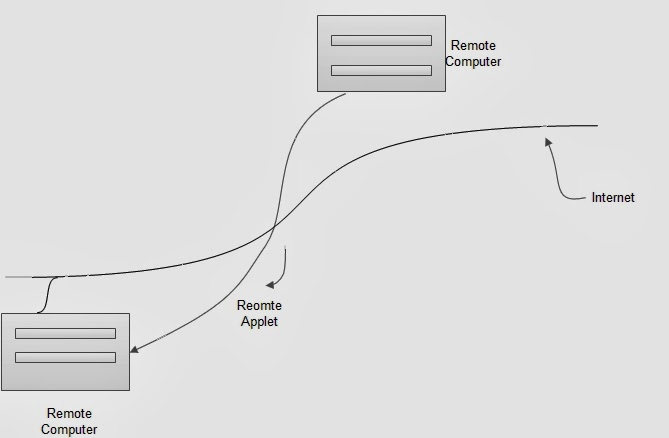
\includegraphics[width=0.45\textwidth]{javaassointernet}
  \caption{Download of applets via internet}
\end{figure}

\section{***Various systems required for internet programming***}
Following are the different system required for internet programming:
\begin{itemize}
  \item Internet Connection
  \item Web-server
  \item HTML
  \item APPLET tag
  \item Java code
  \item Byte code
  \item Proxy server
  \item Mail server
\end{itemize}

\section{Java API}
There are libraries of compiled code that can be used in a program. In other
words, the Java API consist of the function and variables, that programmers
are allowed us access to their application.

\section{Why is Java secure?}
Java is secure due to the following reasons:
\begin{itemize}
  \item Java programs run inside a virtual machine which is known as a
    sandbox.
  \item Java does not support explicit pointer.
  \item Byte-code verifier checks the code fragments for illegal code that can
    violate access right to object.
  \item It provides java.security package implements explicit security.
  \item It provides library level safety.
  \item Run-time security check takes place when we load new code.
\end{itemize}
Java provides some other features that make Java more secure.

\begin{itemize}
  \item JVM
  \item Security API's
  \item Security Manager
  \item Auto Memory Management
  \item No Concept of Pointers
  \item Compile-time Checking
  \item Cryptographic Security
  \item Java Sandbox
  \item Exception Handling
  \item ClassLoader
\end{itemize}

\begin{table}[h]
  \resizebox{\columnwidth}{!}{%
    \begin{tabular}{p{0.4cm}p{2cm}p{3.3cm}p{2cm}}
    \toprule
    & \textbf{Name} & \textbf{Description} & \textbf{Example}\\
    \cmidrule{2-4}
    + & Addition & Adds together two values & x+y\\
    \midrule
    - & Subtraction & Subtracts one value from another & x-y\\
    \midrule
    * & Multiplication & Multiplies two values & x*y\\
    \midrule
    / & Division & Divides one value by another & x/y\\
    \midrule
    \% & Modulus & Return the division remainder & x\%y\\
    \midrule
    ++ & Increment & Increases the value of a variable by 1 & x++\\
    \midrule
    - - & Decrement & Decreases the value of a variable by 1 & - -x\\
    \midrule
    = & Assignment & Assigns value to a variable & x=12\\
    \midrule
    += & Addition assignment & Assigns certain values to itself and asigns the
    total value back to itself & x+=12\\
    \midrule
    ==, >, <, <=, >= & Comparision & Compares two values & x==12, x>10, etc.\\
    \midrule
    \&\&, ||, ! & Logical & Applies logic & x \&\& y, etc.\\
    \bottomrule
  \end{tabular}
}
  \caption{Java Operators}
\end{table}

\section{Java expression}
A Java expression consists of variables, operators, literals, and method
calls.

\noindent\emph{Example}
\begin{verbatim}
  int score;
  score = 90;
\end{verbatim}
Here, \verb+score = 90+ is an expression that returns an int.

Consider another example,

Double \verb+a = 2.2, b = 3.4, result;+
\begin{verbatim}
  result = a + b - 3.4;
\end{verbatim}
Here, \verb|a + b - 3.4| is an expression.

\subsection{Relational Expression}
A relational-expression indicates the condition that the system evaluates.

The syntax is
\begin{verbatim}
variable1 relation_operator variable2;
\end{verbatim}
\noindent\emph{Example}
\begin{verbatim}
  var1 == var2var1 > var2
\end{verbatim}

\subsection{Logical Expression}
A logical expression is a statement that can either be true or false.

The syntax is \verb+condition1 && condition2+
\begin{verbatim}
if(condition1 && condition2)
  d= a + b + c
\end{verbatim}
\noindent\emph{Example}
\begin{lstlisting}
if ((a<b) && (b==c)) {
  d = a + b + c;
  System.out.println("The sum is: " + d);
}
\end{lstlisting}

\subsection{Boolean Expression}
A boolean expression is a Java expression that returns a boolean value: true
or false.

This is useful when we want to compare values to find answers.

\noindent\emph{Example}
\begin{lstlisting}
int x = 10;
int y = 9;
System.out.println(x > y); //returns true
\end{lstlisting}

\section{Control Statements}
Java language processes decision-making capabilitites and supports the
following statement known as control or decision-making statement.

\subsection{If statement}
The \texttt{if} statement is a powerful decision-making statement and is used
to control the following of execution of statement. It is basically a two-way
decision statement and is used in conjunction with the expression. It takes
the following forms
\begin{lstlisting}
if(text expression) {
  statement block;
}
statement x;
\end{lstlisting}
\vskip10pt
\textbf{Example:}
\begin{lstlisting}
...............
...............
if(a > 10) {
  m += 5;
}
System.out.println(m);
...............
...............
\end{lstlisting}

\subsection{Switch statement}
Java has a built-in multiway decision statement known as a switch. The switch
statement test the value of a given variable against a list of cause values
and when a match is found, a block of statements associates with that case is
executed. The general form of the switch statement is as follows
\begin{lstlisting}
switch(expression) {
  case value_1:
    block_1;
    break;
  case value_2:
    block_2;
    break;
  ........
  ........
  default:
    default_block;
    break;
}
statement_x;
\end{lstlisting}

\subsection{Conditional operator statement}
Conditional operator is useful for making two way decision. This operator is a
combination of `?' and `:' and takes three operands. The general form of
conditional statements are as follows

\noindent\texttt{conditional expression ? expression 1 : expression 2;}

Conditional expression. Otherwise expression 2 is evaluated, and its value is
returned

\vskip10pt
\noindent\textbf{Example:}
\begin{lstlisting}
if(x < 0)
  flag = 0;
else
  flag = 1;
\end{lstlisting}
can be written as
\begin{lstlisting}
flag = (x < 0) ? 0 : 1;
\end{lstlisting}

\section{Looping in Java}
In looping a sequence of statement are executed until some condition for the
termination of the loop are satisfied. Depending on the position of the
control statement on the loop, a control structure may be classified either as
the entry control loop or an exit control loop. Java language provides three
contruct for performing loop operation. They are

\subsection{While statement}
The simplest of all the looping stature of Java in the while statement. The
basic formal of the while statement is
\begin{lstlisting}
Initialisation;
while(test condition) {
  body of the loop;
}
\end{lstlisting}
The while is an entry control loop statement. The test condition is evaluated
and if the condition is true, then the body of loop is executed.

\vskip10pt
\noindent\textit{Example}
\begin{lstlisting}
.............
.............
i = 1;
while(i < 10)
{
  System.out.println("i=" + 1);
  i = i + 1;
}
.............
.............
\end{lstlisting}


\subsection{The do-while loop}
The do-while statement is a exit control loop (\textit{The body of the loop
executed at-least once if condition fails}). Since the test condition is
evaluated at the bottom of the loop the do-while construct and provides an
exit control loop and therefore the body of the loop is always executed
at-least once. It takes the following form:

\begin{lstlisting}
Initialisation;
do {
  Body of the loop;
} while(test condition);
\end{lstlisting}

\vskip20pt
\noindent\textit{Example}
\begin{lstlisting}
.............
.............
i = 1;
do {
  System.out.println("i=" + i);
  i = i + 1;
} while(i < 10);
.............
.............
\end{lstlisting}

\subsection{The for statement}
The for loop is another entry control loop that provides a more concise loop
control structure. The general form of the for loop is
\begin{lstlisting}
for(initialization; condition; incrmnt) {
  Body of the loop;
}
\end{lstlisting}

\section{***Array***}
An array is a collection of items of same data type stored at contiguous
memory locations.

This makes it easier to calculate the position of each element by simply adding
an offset to a base value, i.e., the memory location of the first element of
the array (generally denoted by the name of the array). The base value is index
0 and the difference between the two indexes is the offset.

Arrays are classified into 3 main categories. These are:
\subsection{Single dimensional array}
Single indexed variables is referred to a one dimensional or linear array.

\noindent\textbf{Syntax}
\begin{lstlisting}
data_type array_name[] = new data_type[size];
\end{lstlisting}
\noindent\emph{Example}
\begin{lstlisting}
int num[] = new int[5];
\end{lstlisting}

\subsubsection{Program implementation}
\begin{lstlisting}
import java.util.*;

public class oneDarray {
  public static void main(String[] args) {
    Scanner sc = new Scanner(System.in);
    int a[], n;
    System.out.println("Enter how many number");
    n = sc.nextInt();
    a = new int[n];
    System.out.println("Enter array elements:");
    for(int i = 0; i < n; i++) {
      a[i]=sc.nextInt();
    }
    System.out.println("Array elements are:");
    for(int i = 0; i < n; i++) {
      System.out.println(a[i]+" ");
    }
  }
  static void getArr() {
    System.out.println("Enter array elements:");
  }
}
\end{lstlisting}

\subsection{Two dimensional array}
Double indexed variable is referred to as Two dimensional array.

\noindent\textbf{Syntax}
\begin{lstlisting}
data_type array_name[][] = new data_type[r][c];
                            //r = row ; c = column
\end{lstlisting}
\noindent\emph{Example}
\begin{lstlisting}
int num[][] = new int[3][4];
\end{lstlisting}

\subsubsection{Program implementation}
\begin{lstlisting}
import java.util.*;

public class twoDarray {
  public static void main(String[] args) {
    Scanner sc = new Scanner(System.in);
    int a[][], n, m;

    System.out.println("Enter array row");
    n = sc.nextInt();
    System.out.println("Enter array column");
    m = sc.nextInt();

    a = new int[n][m];
    System.out.println("Enter elements: ");
    for(int i = 0; i < n; i++) {
      for(int j = 0; j < m; j++) {
        a[i][j]=sc.nextInt();
      }
    }
    System.out.println("Array elements are: ");
    for(int i = 0; i < n; i++) {
      for(int j = 0; j < m; j++) {
        System.out.println(a[i][j]+" ");
      }
      System.out.println("");
    }
  }
}
\end{lstlisting}
\subsection{Multi-dimensional array}
Multi-dimensional arrays can be defined in simple words as array of arrays.
Data in multi-dimensional arrays are stored in tabular form.

\noindent\textbf{Syntax}
\begin{lstlisting}
data_type[1st dimension][2nd dimension]...[n];
\end{lstlisting}
\vskip10pt
\noindent\emph{Example}
\begin{lstlisting}
array_name = new data_type[1][2]...[n];
\end{lstlisting}

\section{Java Tokens}
A token is the smallest element of a program that is meaningful to the
compiler. Tokens can be classified as follows:

\subsubsection{Keywords}
Keywords are pre-defined or reserved words in a programming language. Each
keyword is meant to perform a specific function in a program. Since
keywords are referred names for a compiler, they can’t be used as variable
names because by doing so, we are trying to assign a new meaning to the
keyword which is not allowed. Java language supports following keywords:
\begin{table}[ht]
\resizebox{\columnwidth}{!}{
\begin{tabular}{|llllll|}
  \toprule
  abstract    & assert     & boolean &
  break       & byte       & case\\\midrule
  catch       & char       & class &
  const       & continue   & default\\\midrule
  do          & double     & else &
  enum        & exports    & extends\\\midrule
  final       & finally    & float &
  for         & goto       & if\\\midrule
  implements  & import     & instanceof &
  int         & interface  & long\\\midrule
  module      & native     & new &
  open        & opens      & package\\\midrule
  private     & protected  & provides &
  public      & requires   & return\\\midrule
  short       & static     & strictfp &
  super       & switch     & synchronized\\\midrule
  this        & throw      & throws &
  to          & transient  & transitive\\\midrule
  try         & uses       & void &
  volatile    & while      & with\\\bottomrule
\end{tabular}
}
\end{table}

\subsubsection{Identifiers}
Identifiers are used as the general terminology for naming of variables,
functions and arrays. These are user-defined names consisting of an
arbitrarily long sequence of letters and digits with either a letter or the
underscore (\_) as a first character. Identifier names must differ in
spelling and case from any keywords. You cannot use keywords as
identifiers; they are reserved for special use. Once declared, you can use
the identifier in later program statements to refer to the associated
value. A special kind of identifier, called a statement label, can be used
in goto statements.

\subsubsection{Constants}
Constants are also like normal variables. But, the only difference is,
their values can not be modified by the program once they are defined.
Constants refer to fixed values. They are also called as literals.
Constants may belong to any of the data type.

\subsubsection{Special Symbols}
The following special symbols are used in Java having some special meaning
and thus, cannot be used for some other purpose.

\subsubsection{Operators}
Java provides many types of operators which can be used according to the
need. They are classified based on the functionality they provide. Some of
the types are
\begin{itemize}
  \item Arithmetic Operators
  \item Unary Operators
  \item Assignment Operator
  \item Relational Operators
  \item Logical Operators
  \item Ternary Operator
  \item Bitwise Operators
  \item Shift Operators
  \item instance of operator
  \item Precedence and Associativity
\end{itemize}
\vskip20pt
%}}}

\begin{tcolorbox}%{{{
  \part{Unit 2}
\end{tcolorbox}
\section{Class}
In object-oriented programming, a class is a basic building block. It can be
defined as template that describes the data and behaviour associated with the
class instantiation. Instantiating is a class is to create an object
(variable) of that class that can be used to access the member variables and
methods of the class.

Following are the different types of classes in Java:
\subsection{Pre-defined}
\begin{itemize}
  \item Scanner
  \item Console
  \item System
  \item String
\end{itemize}
\subsection{User-defined}
A class which is created by a programmer is called user-defined class.

\vskip10pt
\noindent\emph{Example}
\begin{lstlisting}
Class class_name {
  // Data
  // Methods
}
\end{lstlisting}

\section{Objects}
Objects are key to understanding object-oriented technology. The purpose of
the object-oriented programming is to implement the real word entities in
programming. It also emphasis on the binding of data. There are various OOPs
concepts among them Object is one of them. In this section, we will discuss
the object definition in Java.

\vskip10pt
\noindent\textbf{Syntax}
\begin{lstlisting}
class_name obj_name = new class_name();
\end{lstlisting}

\noindent\emph{Example}
\begin{lstlisting}
class demo {
  int a = 10;
  String b = "swapnil";
  void show() {
    System.out.println(a+" "+b);
  }
}

class ob {
  public static void main(String[] agrs) {
    demo r = new demo();
    r.show();
  }
}
\end{lstlisting}

\section{Polymorphism}
Polymorphism means that `same object having different behaviour'

Types of polymorphism:
\subsection{Compile-time polymorphism}
A polymorphism that exist at the time of compilation is called compile-time
polymorphism, it is also known as static polymorphism.
\subsubsection{Method overloading}
When there are multiple functions with the same name but different parameters
then these functions are said to be overloaded. Functions can be overloaded by
change in the number of arguments or/and a change in the type of arguments.

\noindent\emph{Example}
\begin{lstlisting}
class A {
  void add() {
    int a = 10, b = 20, c;
    c = a + b;
    System.out.println(c);
  }
  void add(int x, int y) {
    int c;
    c = x + y;
    System.out.println(c);
  }
  void add(int x, double y) {
    double c;
    c = x + y;
    System.out.println(c);
  }
}
public class overload {
  public static void main(String[] args) {
    A r = new A();
    r.add();
    r.add(20, 34);
    r.add(32, 3.456);
  }
}
\end{lstlisting}

\subsection{Run-time polymorphism}
A polymorphism which exist at the time of execution of program is called
runtime polymorphism.

\subsubsection{Method overriding}
Whenever we writing method in super and sub classes in such a way that method
name and parameter must be same called method overriding.

\noindent\emph{Example}
\begin{lstlisting}
class shape {
  void draw() {
    System.out.println("cant say shape type");
  }
}
class square extends shape {
  void draw() {
    System.out.println("square shape");
  }
}
class demo {
  public static void main(String[] args) {
    shape r = new square();
    r.draw();
  }
}
\end{lstlisting}

\begin{table}[ht]
  \resizebox{\columnwidth}{!}{
    \begin{tabular}{lp{3.4cm}p{3.4cm}}
      \toprule
      & Method Overloading & Method Overriding\\
      \cmidrule{2-3}
      1 &
        Whenever a class contain more than one
        method with same and different types of
        parameters called method overloading. &
        Whenever we writing method in super and
        sub classes in such a way that method name
        and parameter must be same called method
        overriding.\\
      \midrule
      2 &
        This is relationship between methods in a
        same class. &
        This is relationship between superclass
        method and subclass method.\\
      \midrule
      3 &
        May have different return data type. &
        Must have same return type.\\
      \midrule
      4 &
        This is an example of compile time
        polymorphism. &
        This is an example of run time
        polymorphism. \\
        \bottomrule
    \end{tabular}
  }
  \caption{Difference between method overloading and overriding}
\end{table}

\section{***Java Constructor***}
Constructor is a special type of method whose name is same as class name.
\begin{enumerate}
  \item The main purpose of constructor is initialize the object.
  \item Every Java class has constructor.
  \item A constructor is automatically called at the time of object creation.
  \item A constructor never contain any return type including void.
\end{enumerate}

\noindent\emph{Example}
\begin{lstlisting}
class A {
  int a;
  String name;
  A() {
    a = 0;
    name = null;
  }
  void show() {
    System.out.println(a + " " + name);
  }
}
class B {
  public static void main(String[] args) {
    A ref = new A();
    ref.show();
  }
}
\end{lstlisting}

\section{***Constructor Overloading***}
Whenever we have more than one constructor in out class then it is called
constructor overloading.

\noindent\emph{Example}
\begin{lstlisting}
class con {
  int a;
  double b;
  String c;
  con() {
    a = 100;
    b = 45.45;
    c = "masuk";
  }
  con(int x) {
    a = x;
  }
  con(double y, String z) {
    b = y;
    c = z;
  }
}
public class Construc {
  public static void main(String[] args) {
    con r = new con();
    con r2 = new con(10);
    con r3 = new con(23.56, "mass");
    System.out.println(r.a+" "+r.b+" "+r.c);
    System.out.println(r2.a);
    System.out.println(r3.b+" "+r3.c);
  }
}
\end{lstlisting}

\section{***Inheritance***}
In Java, inheritance means creating new classes based on existing ones. A
class that inherits from another class can reuse the methods and fields of
that class. In addition, you can add new fields and methods to your current
class as well.
\subsection{Types of inheritance}
\subsubsection{Single level inheritance}
In single inheritance, subclasses inherit the features of one superclass. In
the image below, class A serves as a base class for the derived class B.

\begin{figure}
  \centering
  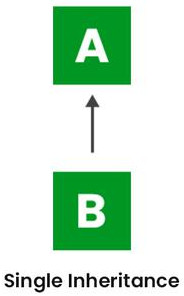
\includegraphics[width=0.7\columnwidth]{singlevin}
  \caption{Single level inheritance}
\end{figure}

\vskip20pt
\noindent\emph{Example}
\begin{lstlisting}
class A {
  void disp_A() {
    System.out.println("Display A");
  }
}
class B extends A {
  void disp_B() {
    System.out.println("Display B");
  }
}
public class singleinh {
  public static void main(String[] args) {
    B b = new B();
    b.disp_A();
    b.disp_B();
  }
}
\end{lstlisting}

\subsubsection{Multi level inheritance}
In Multilevel Inheritance, a derived class will be inheriting a base class,
and as well as the derived class also acts as the base class for other
classes. In the below image, class A serves as a base class for the derived
class B, which in turn serves as a base class for the derived class C. In
Java, a class cannot directly access the grandparent’s members.

\begin{figure}[h]
  \centering
  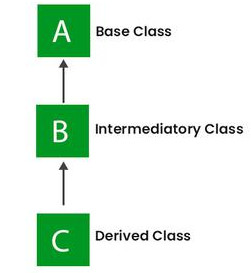
\includegraphics[width=0.8\columnwidth]{mullevin}
  \caption{Multi level inheritance}
\end{figure}

\vskip20pt
\noindent\emph{Example}
\begin{lstlisting}
class A //super class
{
  void disp_A() {
    System.out.println("Display A");
  }
}
class B extends A //Intermediate base class
{
  void disp_B() {
    System.out.println("Display B");
  }
}
class C extends B //child class
{
  void disp_C() {
    System.out.println("Display C");
  }
}
public class multilvl {
  public static void main(String[] args) {
    C c = new C();
    c.disp_A();
    c.disp_B();
    c.disp_C();
  }
}
\end{lstlisting}

\subsubsection{Why multiple inheritance not supported in Java?}
Whenever a sub class wants to inherit the property of two or more super class
that have same method, Java compiler can't decide which class method it should
inherit.

\begin{figure}[h]
  \centering
  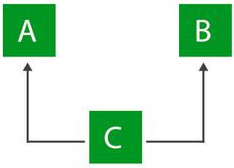
\includegraphics[width=0.8\columnwidth]{multiin}
  \caption{Multiple inheritance}
\end{figure}

Then their might be a chance of memory duplication i.e a reason Java doesn’t
support multiple inheritance through classes.
Consider a case where class B extends class A and Class C and both class A and
C have the same method \verb+display()+.
Now java compiler cannot decide, which display method it should inherit. To
prevent such situation, multiple inheritances is not allowed in java.

\section{***Muliple Inheritance implementation using interface***}
We can achieve multiple inheritance through interfaces because interface
contains only abstract method, which implementation is provided by the sub
classes.

\vskip20pt
\noindent\emph{Example}
\begin{lstlisting}
interface A {
  void show();
}
interface B {
  void show();
}
class Multiple implements A, B {
  public void show() {
    System.out.println("Interface A & B");
  }
  public static void main(String[] args) {
    Multiple m = new Multiple();
    m.show();
  }
}
\end{lstlisting}

\section{Package}
A package arrange number of classes, interfaces and sub-package of same type
into a particular group. Package is nothing but folder like windows folder
where we can store same type of data.
\subsection{Types of packages}
\subsubsection{Pre-defined}
\begin{itemize}
  \item java.lang
  \item java.util
  \item java.io
  \item java.awt
  \item java.applet
  \item java.net
  \item java.SQL
\end{itemize}
\subsubsection{User-defined}
User define package is created with the help of the `package' keyword. Whereas
to use a we use the import keyword.

\subsection{Advantages}
\begin{itemize}
  \item Reusability
  \item Security
  \item Fast searching
  \item Naming conflicting
  \item Hiding.
\end{itemize}

\section{Garbage Collection in Java}
In Java, garbage means unreferenced objects.
Garbage collection is process of reclaiming the runtime unused memory
automatically. In other worsds, it is away to destroy the unused objects.

The Garbage collector of JVM collects only those objects that are created by
new keyword. So if we have create any object without new, we can use finalize
method to perform cleanup processing (destroying remaining objects).

\section{Finalize Method}
Finalize is a method, which is available in object super class. The purpose of
the finalize method is to release the resources that is allocated by unused
object, before removing unused object by garbage collector.

\section{Why class path is necessary}
%}}}

\begin{tcolorbox}%{{{
  \part{Unit 3}
\end{tcolorbox}
\section{Exception Handling}
Exception handling is a mechanism to handle runtime errors, so that normal
flow of the program can be maintained.

\subsection{Advantages}
\begin{itemize}
  \item Using exception handling we can separate the error handling code from
    normal code.
  \item Using exception handling we can differentiate the error types.
  \item Normal flow of the program can be maintained.
\end{itemize}

\subsection{Types of Exception}
\subsubsection{Checked Exception}
Checked exceptions are those exceptional conditions that are checked by
compiler at the compile time. A checked exception forces you to either use
try-catch or throws. All exceptions except Error, RuntimeException, and their
subclasses are checked exceptions. e.g. IOException, SQLException etc.
\subsubsection{Unchecked Exception}
Unchecked exceptions are those exceptional conditions that are not checked by
compiler at the compile time. Unchecked exceptions are checked at runtime. An
unchecked exception not forces you to either use try-catch or throws.
RuntimeException and their subclasses are unchecked exceptions. This exception
can be avoided by programmer. e.g. NullPointerException, ArithmeticException
etc.

\newpage
\noindent\emph{Example}
\begin{lstlisting}
import java.util.*;

public class demoException2 {
  public static void main(String[] args) {
    Scanner in = new Scanner(System.in);
    try {
      int a[] = new int[5];
      String s = null;
      System.out.println(s.length());
    } catch (ArithmeticException e) {
      System.out.println("Arithmetic Exception
                            occurs");
    } catch (ArrayIndexOutOfBoundsException e) {
      System.out.println("ArrayIndexOutOfBounds
                            Exception occurs");
    } catch (NullPointerException e) {
      System.out.println("Null Pointer Exception");
    }
    System.out.println("rest of the code");
  }
}
\end{lstlisting}

\section{Multithreading}
The process of executing multiple tasks (also called threads) simultaneously
is called multithreading. The primary purpose of multithreading is to provide
simultaneous execution of two or more parts of a program to make maximum use
of CPU time. A multithreaded program contains two or more parts that can run
concurrently. It enables programmers to write in a way where multiple
activities can proceed simultaneously within a single application.

\subsection{How to create thread in Java run with example.}
Creating thread in Java is simple. Thread are implemented in the form of
objects that contains a method called \verb+run()+ method. The \verb+run()+ is
the heart and soul of any thread. It makes up the entire body of a thread and
is the only method in which the threads behaviour can be implemented. A
typical \verb+run()+ method would appear as follows:
\begin{lstlisting}
public void run() {
  // statement for implementing thread.
}
\end{lstlisting}

\noindent\emph{Example}
\begin{lstlisting}
class A extends Thread {
  public void run() {
    for (int i = 1; i <= 5; i++) {
      System.out.println("From thread A : i = "+i);
    }
    System.out.println("Exit from A");
  }
}
class B extends Thread {
  public void run() {
    for (int j = 1; j <= 5; j++) {
      System.out.println("From thread B : j = "+j);
    }
    System.out.println("Exit from B");
  }
}
class c extends Thread {
  public void run() {
    for (int k = 1; k <= 5; k++) {
      System.out.println("From thread C : k = "+k);
    }
    System.out.println("Exit from C");
  }
}
class thread Test {
  public static void main(String[] args) {
    new A().start();
    new B().start();
    new C().start();
  }
}
\end{lstlisting}

\subsection{Life cycle of a thread}
During the life time of a thread there are many step they enter this include:
\begin{itemize}
  \item Newborn/ New Thread state
  \item Runnable state
  \item Running state
  \item Block state
  \item Dead state
\end{itemize}
\begin{figure}[h]
  \centering
  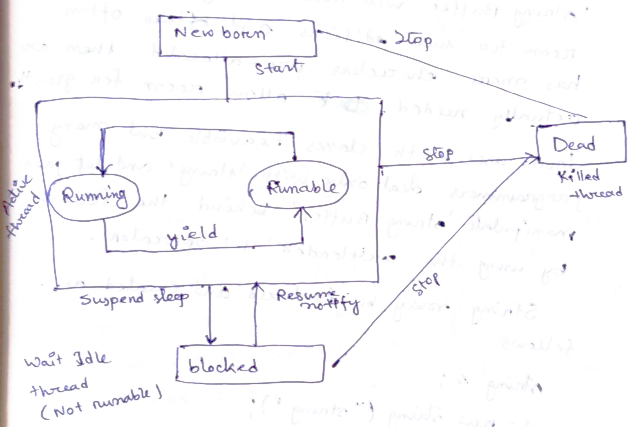
\includegraphics[width=\columnwidth]{strandiagtrd}
  \caption{State transition diagram of a thread}
\end{figure}

\begin{table}[ht]
  \resizebox{\columnwidth}{!}{
    \begin{tabular}{p{1.4cm}p{3cm}p{3cm}}
      \toprule
      \textbf{Basis for Comparison} & \textbf{Thread} & \textbf{Runnable} \\
      \midrule
      Basic &
        Each thread creates a unique object and gets associated with it. &
        Multiple threads share the same objects. \\\midrule
      Memory &
        As each thread create a unique object, more memory required. &
        As multiple threads share the same object less memory is used.\\
        \midrule
      Extending &
        In Java, multiple inheritance not allowed hence, after a class extends
        Thread class, it can not extend any other class. &
        If a class define thread implementing the Runnable interface it has a
        chance of extending one class.\\\midrule
      Use &
        A user must extend thread class only if it wants to override the other
        methods in Thread class. &
        If you only want to specialize run method then implementing Runnable
        is a better option. \\\midrule
      Coupling &
        Extending Thread class introduces tight coupling as the class contains
        code of Thread class and also the job assigned to the thread &
        Implementing Runnable interface introduces loose coupling as the code
        of Thread is separate form the job of Threads.\\
      \bottomrule
    \end{tabular}
  }
  \caption{Difference between thread and runnable interface}
\end{table}

\section{Autoboxing}
It is the automatic conversion that java compiler makes between the primitive
types and their corresponding object Wrapper classes.

\noindent\emph{Example}
\begin{lstlisting}
class BoxingExample1 {
  public static void main(String args[]) {
    int a = 50;
    Integer a2 = new Integer(a); //Boxing
    Integer a3 = 5; //Boxing
    System.out.println(a2 + " " + a3);
  }
}
\end{lstlisting}
\section{Unboxing}
The automatic conversion of wrapper class type into corresponding primitive
type is known as unboxing

\noindent\emph{Example}
\begin{lstlisting}
class UnboxingExample1 {
  public static void main(String args[]) {
    Integer i = new Integer(50);
    int a = i;
    System.out.println(a);
  }
}
\end{lstlisting}

\section{Abstract Class}
A class which is declared with the abstract keyword is known as an abstract
class in Java. It can have abstract and non-abstract methods (method with the
body)

\section{***Interface***}
Interface is just like a class, which contains only abstract method. To
achieve interface java provides a keyword called `implements'.
\begin{itemize}
  \item Interface method are by default public \& abstract.
  \item Interface variables are by default public+ static + final.
  \item Interface method must be overridden inside the implementing classes.
\end{itemize}

\noindent\emph{Example}
\begin{lstlisting}
interface Area {
  final static float pi = 3.14 F;
  float compute(float x, float y);
  String compute(double d, double e);
}
class Rectangle implements Area {
  public float compute(float x, float y) {
    return (x * y);
  }
}
class Circle implements Area {
  public float compute(float x, float y) {
    return (pi * x * x);
  }
}
class interface Test {
  public static void main(String[] args) {
    Rectangle rect = new Rectangle();
    Circle cir = new Circle();
    Area area;
    area = rect;
    System.out.println("Area of Rectangle"
                          +area.compute(3.5, 5));
    area = cir;
    System.out.println("Area of circle"
                          +area.compute(10, 0));
  }
}
\end{lstlisting}

\begin{table}[ht]
  \resizebox{\columnwidth}{!}{
    \begin{tabular}{lp{3cm}p{3cm}}
      \toprule
      & \textbf{Abstract Class} & \textbf{Interface} \\
      \cmidrule{2-3}
      1. &
        To declare an abstract class we use abstract keyword. &
        To declare an interface we use interface keyword.\\
      \midrule
      2. &
        A class extend only one abstract class. &
        A class implement more than one interfaces. \\
      \midrule
      3. &
        In abstract class relationship we say A in B. &
        In interface relationship we say A has C, D, \& E. \\
      \bottomrule
    \end{tabular}
  }
  \caption{Difference between abstract class and interface.}
\end{table}

\begin{table}[ht]
  \resizebox{\columnwidth}{!}{
    \begin{tabular}{lp{3.5cm}p{3.5cm}}
      \toprule
      & \textbf{Class} & \textbf{Interface}\\
      \cmidrule{2-3}
      1. &
        The member of a class can be constants or variable. &
        The member of inface are always declared as constant i.e. their values
        are final.\\
      \midrule
      2. &
        The class definition can contain the code for each of its method IE
        methods can be abstract or non-abstract. &
        The method in an interface are abstract in value i.e. there is no code
        associated with them. \\
      \midrule
      3. &
        It can be initiated by declaring object. &
        It cannot be use to declare object. \\
      \midrule
      4. &
        It can use various access specifiers like public, private, protected.
        &
        It can only use the public access specifier. \\
      \bottomrule
    \end{tabular}
  }
  \caption{Difference between class and interface.}
\end{table}
%}}}

\begin{tcolorbox}%{{{
  \part{Unit 4}
\end{tcolorbox}

\section{***Applet life-cycle***}
In java, an applet is a special type of program embedded in the web page to
generate dynamic content. Applet is a class in Java. The applet life cycle can
be define as the process of how the object is created, started, stopped, and
destroyed during the entire execution of its application. It basically has
five core method namely \verb+init()+, \verb+start()+, \verb+stop()+,
\verb+paint()+, and \verb+destroy()+. These methods are invoked by the browser
to execute.

\begin{figure}[ht]
  \centering
  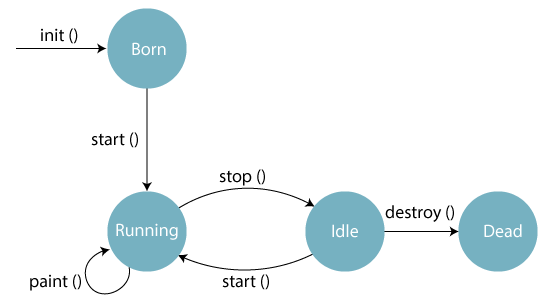
\includegraphics[width=\columnwidth]{appletlc}
  \caption{Applet Life Cycle}
\end{figure}
There are five methods of an applet life cycle, and they are:

\subsubsection{\texttt{init()}}
The \verb+init()+ method is the first method to run that initializes the
applet. It can be invoked only once at the time of initialization. The web
browser creates the initialized objects, i.e., the web browser (after checking
the security settings) runs the \verb+init()+ method within the applet.

\subsubsection{\texttt{start()}}
The \verb+start()+ method contains the actual code of the applet and starts
the applet. It is invoked immediately after the \verb+init()+ method is
invoked. Every time the browser is loaded or refreshed, the \verb+start()+
method is invoked. It is also invoked whenever the applet is maximized,
restored, or moving from one tab to another in the browser. It is in an
inactive state until the \verb+init()+ method is invoked.

\subsubsection{\texttt{stop()}}
The \verb+stop()+ method stops the execution of the applet. The \verb+stop()+
method is invoked whenever the applet is stopped, minimized, or moving from
one tab to another in the browser, the \verb+stop()+ method is invoked. When
we go back to that page, the \verb+start()+ method is invoked again.

\subsubsection{\texttt{destroy()}}
The \verb+destroy()+ method destroys the applet after its work is done. It is
invoked when the applet window is closed or when the tab containing the
webpage is closed. It removes the applet object from memory and is executed
only once. We cannot start the applet once it is destroyed.

\subsubsection{\texttt{paint()}}
The \verb+paint()+ method belongs to the Graphics class in Java. It is used to
draw shapes like circle, square, trapezium, etc., in the applet. It is
executed after the \verb+start()+ method and when the browser or applet
windows are resized.

\section{***Difference between AWT and Swing.***}
\begin{itemize}
  \item Swing components sits on the top of AWT components and do the work.
  \item AWT components are called heavy weight components and swing are called
    light weight components.
  \item Swing components made in purely Java and they are platform independent
    where as AWT components are platform dependent.
  \item The appearance of AWT components is mainly not configurable. It
    generally depends on the operating system’s look and feels. Where the
    swing components are configurable and mainly support pluggable look and
    feel.
  \item Java AWT is slower than swing in terms of performance. Where Java
    Swing is faster than the AWT.
\end{itemize}

\section{***Java Applet program to add and multiply two numbers using two
TextBoxes and Buttons***}
\begin{lstlisting}
import java.applet.*;
import java.awt.*;
import java.awt.event.*;

public class appMul extends Applet implements
                                       ActionListener {
  TextField t1 = new TextField(10);
  TextField t2 = new TextField(10);
  TextField t3 = new TextField(10);
  TextField t4 = new TextField(10);

  Label l1 = new Label("FIRST NO=:");
  Label l2 = new Label("SECOND NO:");
  Label l3 = new Label("SUM:");

  Button b = new Button("Calculate Sum and
                            Product");
  Label l4 = new Label("Multiplication:");

  public void init() {
    add(l1);
    add(t1);
    add(l2);
    add(t2);
    add(l3);
    add(l4);
    add(t3);
    add(t4);
    add(b);
    b.addActionListener(this);
  }

  public void actionPerformed(ActionEvent e) {
    if (e.getSource() == b) {
      int n1 = Integer.parseInt(t1.getText());
      int n2 = Integer.parseInt(t2.getText());
      t3.setText(" " + (n1 + n2));
      t4.setText(" " + (n1 * n2));
    }
  }
}
\end{lstlisting}

\subsubsection{Write an applet program to display the message hello world in
the applet windows at position (20, 30) or (how to run applet program).}
First we write the applet code as:
\begin{lstlisting}
import java.applet.Applet;
import java.awt.Graphics;
public class First extends Applet {
  public void point(Graphics g) {
    g.drawString("hello world", 150, 150);
  }
}

<html>
  <body>
    <applet code="First class" height=20, width=30>
    </applet>
  </body>
</html>
\end{lstlisting}

To run the above applet code:
\begin{verbatim}
C:\javac First.java
C:\appletviewer First.java
\end{verbatim}

\begin{figure}[h]
  \centering
  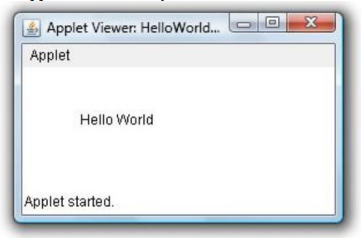
\includegraphics[width=\columnwidth]{apletviewer}
\end{figure}

\section{***Layout manager***}
The LayoutManagers are used to arrange components in a particular manner. The
Java LayoutManagers facilitates us to control the positioning and size of the
components in GUI forms. LayoutManager is an interface that is implemented by
all the classes of layout managers. There are the following classes that
represent the layout managers:
\begin{lstlisting}
java.awt.BorderLayout
java.awt.FlowLayout
java.awt.GridLayout
java.awt.CardLayout
java.awt.GridBagLayout
javax.swing.BoxLayout
\end{lstlisting}

\subsubsection{BorderLayout}
The BorderLayout is used to arrange the components in five regions: north,
south, east, west, and center. Each region (area) may contain one component
only.
\begin{lstlisting}
public static final int NORTH
public static final int SOUTH
public static final int EAST
public static final int WEST
public static final int CENTER
\end{lstlisting}

\vskip10pt
\noindent\emph{Example}
\begin{lstlisting}
f = new JFrame();

JButton b1 = new JButton("NORTH");;
// the button will be labeled as NORTH

JButton b2 = new JButton("SOUTH");;
// the button will be labeled as SOUTH
\end{lstlisting}
\subsubsection{GridLayout}
The Java GridLayout class is used to arrange the components in a rectangular
grid. One component is displayed in each rectangle.

\vskip10pt
\noindent\emph{Example}
\begin{lstlisting}
f = new JFrame();
JButton btn1 = new JButton("1");
JButton btn2 = new JButton("2");
f.add(btn1);
f.add(btn2);
f.setLayout(new GridLayout());
\end{lstlisting}

\subsubsection{FlowLayout}
The Java FlowLayout class is used to arrange the components in a line, one
after another (in a flow). It is the default layout of the applet or panel.
\begin{lstlisting}
public static final int LEFT
public static final int RIGHT
public static final int CENTER
public static final int LEADING
public static final int TRAILING
\end{lstlisting}

\vskip10pt
\noindent\emph{Example}
\begin{lstlisting}
f = new JFrame();
JButton btn1 = new JButton("1");
JButton btn2 = new JButton("2");
f.add(btn1);
f.add(btn2);
f.setLayout(new FlowLayout());
\end{lstlisting}

\subsubsection{CardLayout}
The Java CardLayout class manages the components in such a manner that only one
component is visible at a time. It treats each component as a card that is why
it is known as CardLayout.

\vskip10pt
\noindent\emph{Example}
\begin{lstlisting}
Container cPane = getContentPane();
CardLayout crd = new CardLayout();
cPane.setLayout(crd);
JButton btn1 = new JButton("Apple");
cPane.add("a", btn1);
\end{lstlisting}

\subsubsection{GridBagLayout}
The Java GridBagLayout class is used to align components vertically,
horizontally or along their baseline. The components may not be of the same
size. Each GridBagLayout object maintains a dynamic, rectangular grid of cells.

\vskip10pt
\noindent\emph{Example}
\begin{lstlisting}
GridBagLayout layout = new GridBagLayout();
GridBagConstraints gbc = new GridBagConstraints();
this.setLayout(layout);
gbc.fill = GridBagConstraints.HORIZONTAL;
\end{lstlisting}

\subsubsection{BoxLayout}
The Java BoxLayout class is used to arrange the components either vertically or
horizontally. For this purpose, the BoxLayout class provides four constants.
They are as follows:
\begin{lstlisting}
public static final int X_AXIS:
          Alignment of the components are horizontal
          from left to right.

public static final int Y_AXIS:
          Alignment of the components are vertical
          from top to bottom.

public static final int LINE_AXIS:
          Alignment of the components is similar to
          the way words are aligned in a line
\end{lstlisting}

\vskip10pt
\noindent\emph{Example}
\begin{lstlisting}
setLayout (new BoxLayout (this, BoxLayout.Y_AXIS));
\end{lstlisting}

\subsection{AWT v/s Swing? Which one is light weight component and which one is heavy weight component?}
\subsubsection{AWT:}
It is a Heavy weight component. Because, AWT is said to be "Heavyweight"
because basically each AWT component is a native platform component. AWT is
implemented on top of the platform's native GUI toolkit. This also explains why
AWT was pretty limited compared to Swing.

\subsubsection{Swing:}
It is a light weight component. Because, it is fully implemented in Java,
without calling the native operating system for drawing the graphical user
interface components.

\section{Container in Java}
Containers are the interface between a component and the low-level,
platform-specific functionality that supports the component.
\begin{itemize}
  \item A Container class can be described as a special component that can hold the gathering of the components.
  \item There are two types of Swing Containers, they are top-level containers and low-level containers.
  \item Top-Level containers are heavyweight containers such as JFrame, JApplet, JWindow, and
  \item alog.
  \item Low-Level containers are lightweight containers such as JPanel.
  \item The most commonly used containers are JFrame, JPanel and JWindow.
  \item The important methods of the Container class are add(), invalidate() and validate()
\end{itemize}

\vskip10pt
\noindent\emph{Example}
\begin{lstlisting}
import java.awt.*;
import javax.swing.*;
public class ContainerTest extends JFrame {
  JPanel panel; // low-level container
  JTextField field;
  JButton btn;
  public ContainerTest() {
    setTitle("Container Test");
    panel = new JPanel();
    field = new JTextField(20);
    panel.add(field);
    btn = new JButton("Submit");
    panel.add(btn);
    add(panel, BorderLayout.CENTER);
    setSize(350, 275);
    setDefaultCloseOperation(JFrame.EXIT_ON_CLOSE);
    setLocationRelativeTo(null);
    setVisible(true);
  }
  public static void main(String args[]) {
    new ContainerTest();
  }
}
\end{lstlisting}
%}}}

\begin{tcolorbox}%{{{
  \part{Unit 5}
\end{tcolorbox}
\section{***JDBC***}
Java database connectivity is an application programming interface for the
programming language.java which defines how a client may access a database. It
is a java based data access technology used for java database connectivity. It
is part of the java standard edition platform, from oracle corporation.

The JDBC library includes APIs for each of the tasks mentioned below that are
commonly associated with database usage.
\begin{itemize}
  \item Making a connection to a database.
  \item Creating sql or MySQL statements.
  \item Executing SQL or MYSQL queries in the database.
  \item Viewing \& modifying the resulting record.
\end{itemize}

\subsection{Application JDBC}
Fundamentally JDBC is a specification that provides a complete set of
interfaces that allows for portable access to an underlying database. Java can
be used to write different types of executables such as:
\begin{itemize}
  \item Java application
  \item Java applets
  \item Java servlete
  \item Java server pages (JSPS)
  \item Enterprise java beans(EJBS)
\end{itemize}
All of these different executables are able to use a JDBC driver to access a
database and take advantages of the stored data.

JDBC provides the same capabilities as ODBC allowing java programs to contain
database independent code.

\subsection{Architecture}
The JDBC API supports both two-tier or three tier processing models for
database access but in general JDBC architecture consists of two layers:
\begin{itemize}
  \item JDBC API

    This provides the application to JDBC manager connection.
  \item JDBC Driver API

    This supports the jdbc manager to driver connection.
\end{itemize}
The JDBC API uses a driver manager and database specific drivers to provide
transparent connectivity to heterogeneous database. The JDBC driver manager
ensures that the correct driver is used to access each data source. The driver
manager is capable of supporting multiple concurrent devices connected to
multiple heterogeneous database. Following is the architecture diagram which
shows the location of the driver manager with respect to the JDBC drivers and
the java application:
\begin{figure}[ht]
  \centering
  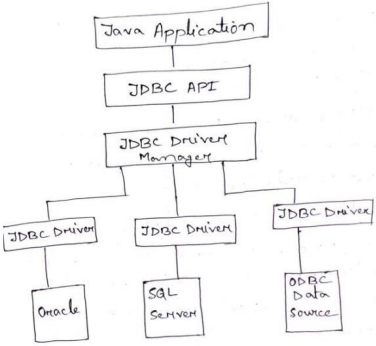
\includegraphics[width=\columnwidth]{jdbcarc}
\end{figure}

\subsection{Different components of JDBC}
\subsubsection{Driver manager}
This class manages a list of database drivers. Matches connection request from
the java application with the proper database driver using communication sub
protocol. The first driver that recognizes a certain sub protocol under JDBC
will be used to establish a database connection.

\subsubsection{Driver}
This interface handles the communications with the database server. We will
interact directly with driver manager objects, which manages objects of this
type. It also abstracts the details associated with working with driver
objects.

\subsubsection{Connection}
This interface with all methods for contracting a database. The connection
object represents communication context i.e. all communication with database is
through connection object only.

\subsubsection{Statement}
We use objects created from this interface to submit the SQL statements to the database. Some derived interfaces accept parameters in addition to executing
stored procedures.

\subsubsection{Result}
These objects hold data retrieved from a database after we execute an SQL query
using statement objects, it acts as an iterator to allow us to move through its
data.

\subsubsection{SQL Exception}
This class handles any errors that occur in a database application.

\subsection{Different JDBC driver}
It is software component that enables java application to interact with the
database. There are four types of JDBC driver:
\subsubsection{JDBC-ODBC bridge driver}
It uses ODBC driver to connect to the database. The JDBC ODBC bridge drivers converts JDBC method calls into the ODBC function calls
\begin{figure}[ht]
  \centering
  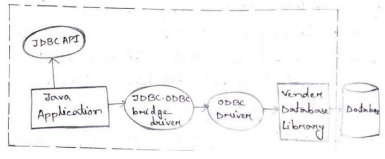
\includegraphics[width=\columnwidth]{jdbcodbc}
  \caption{JDBC-ODBC bridge driver}
\end{figure}

\subsubsection{Native API driver}
The Native API driver uses the Clint side libraries of the database. The driver
converts JDBC method calls into native calls of the database API. It is not
written entirely in java.
\begin{figure}[ht]
  \centering
  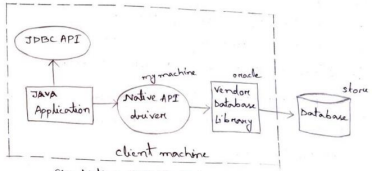
\includegraphics[width=\columnwidth]{jdbcnative}
  \caption{Native API driver}
\end{figure}

\subsubsection{Network protocol driver}
It uses middle ware (application server) that converts JDBC calls directly or
indirectly into the vendor specific database protocol. It is fully written in
java.
\begin{figure}[ht]
  \centering
  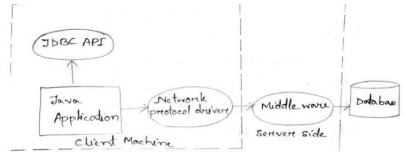
\includegraphics[width=\columnwidth]{jdbcnet}
  \caption{Network protocol driver}
\end{figure}

\subsubsection{Thin driver}
It converts JDBC calls directly into the vendor specific database protocol.
That is why it is known as thin driver. It is fully written in java language.

\begin{figure}[ht]
  \centering
  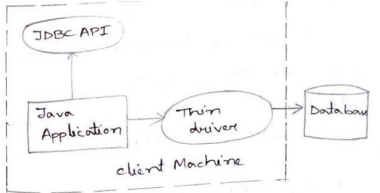
\includegraphics[width=\columnwidth]{jdbcthin}
  \caption{Thin driver}
\end{figure}

\subsubsection{***How database connection can be established through JDBC
(Establishing connectivity and working with connection interface).***}
There are five step to connect any Java application with the database using
JDBC. These steps are as follow:
\begin{itemize}
  \item [\textbf{Step 1}:] Register the Driver class:

    The \verb+forName()+ method of class is used to register the driver class.
    The method is used to dynamically load the driver class.

    Syntax of \verb+forName()+ method
    \begin{lstlisting}
Public static void forName(String className)
    \end{lstlisting}
    throws

    \verb+classNotFound Exception+
    For example, Java program to load oracle driver to establish database
    connection as follows:

    \begin{lstlisting}
Class.forName("oreacle.jdbc.driver
                                   .oracleDriver");
    \end{lstlisting}
  \item [\textbf{Step 2}:] Create connection object:

    The getConnection() method of driver manager class is used to establish
    connection with the database.
    \begin{itemize}
      \item \texttt{public static connection getConnection(String url) throws SQL Exception.}
      \item \texttt{public static connection getConnetion(String url, String
        name, String password)}
    \end{itemize}
    throws SQL Exception.

    For example, To establish connection with the oracle database connection

    \texttt{Con=DriverManager.getconnection("jdbc; oracle;thin;@localhost;1521;xe", "system", "password");}
  \item [\textbf{Step 3}:] Create the statement object:

    The create statement() method of connection interface is used to create
    statement: The object of statement is responsible to execute queries with
    the database.

    \vskip10pt
    Syntex of create statement() method

    Public statement

    Create statement() throws SQL Exception

    e.g. to create the statement object statement statement stmt=con.create statement();

  \item [\textbf{Step 4}:] Execute the query:

    The execute Query() method of statement interface is used to execute
    queries to the database.This method returns the object of Resultset that
    can be used to get all the records of a table.

    \vskip10pt
    Syntax of executeQuery(string sql)throws SQL exception

    Public resultset

    Execute query (string sql)throws SQL exception

    e.g. to execute query
    \begin{lstlisting}
Resultset rs=stmt.executeQuery("
                               select*from emp");
While(rs.next()){
System.out.println(rs.getInt(1)+" "
                     +rs.getStriing(2));
    \end{lstlisting}
  \item [\textbf{Step 5}:] Close the connection object:

    By closing connection object statement and Resultset will be closed
    automatically. The close() method of connection interface is used to close
    the connection

    \vskip10pt
    Syntax of close() method

    Public void close()throws SQLexception

    E.g. To close connection con.close(());
\end{itemize}

\subsubsection{How can we create and execute SQL statement in JDBC. Explain
with example.}
\subsubsection{How to work with result set object? Give example.}
%}}}

\end{document}
